%%%%%%%%%%%%%%%%%%%%%%%%%%%%%%%%%%%%%%%%%%%%%%%%%%%%%%%%
%%%%                                              %%%%%%
%%%%  Author: Name des Autors                     %%%%%%
%%%%                                              %%%%%%
%%%%  Beschreibung:                               %%%%%%
%%%%                                              %%%%%%
%%%%%%%%%%%%%%%%%%%%%%%%%%%%%%%%%%%%%%%%%%%%%%%%%%%%%%%%


\chapter{Swimmer Model}
\label{chap:chapter_2}

\section{Swimmers in Nature}
\label{sec:section_1}


Biomechanical principles give the basis for understanding how a swimming body propels itself through a fluid\cite{mchenry_morphology_2005}, as a swimmer can be defined as
an organism or object that moves by deforming its body in a periodic way. For example, an \textit{ascidian larva} creates
\cite{sawada_biology_2001} tail ondulation by the action of its muscles while swimming. This motion generates hydrodynamic forces and torques on the surface of the body that result in a rate and direction
of motion that are determined by body mass and its spatial distribution. A model accurately incorporating these components should successfully predict the direction, rate, and 
energetic cost of swimming.\par
Swimming bodies can be found in many different environments in the nature. The physics governing swimming in micrometer scale is other fromthe physics of swimming at the macroscopic
scale. The microorganisms are in the region of low Reynolds number, where inertia has a little effect and viscous damping is predominant. The Reynolds number is defined as:

\begin{equation} 
  Re = \frac {\rho UL}{\eta}
\end{equation}

where $\rho$ is the fluid density, $\eta$ is the viscosity and $L$ and $U$ are characteristic velocity and length scales of the flow, respectively.\par

Swimming strategies applied by large animals that run at high Reynolds number, such as fish, snakes, birds or insects(\cite{childress_mechanics_1981},\cite{vogel_life_1996},
\cite{digest_natures}) are not effective at small scales. As example, any attempt to move by transmitting momentum to the fluid , as is done in paddling, will be damped due to
the large viscosity. Hence, microorganisms have developed propulsion strategies that sucessfully overcome drag.



\subsection{Microscopic Swimmers}
\label{sec:section 1}

Microscopic swimmers have various means to create propulsion. It can be as a stiff helix that is rotated by a motor embedded in the cell wall, as in the case of \textit{E.coli}
\cite{berg_bacteria_1973}(Figure~\ref{fig:Bild1}(a)), or it can be a flexible filament undergoing whip-like motions due to the action of molecular motors distributed along the
length of the filament, as in the sperm of many species\cite{blum_biophysics_1973} (Figure~\ref{fig:Bild1} (e) and (f)). Bacterias can swimm in different manners, for example, 
\textit{Caulobacter Crescentus}  has a single right-handed helical filament(Figure~\ref{fig:Bild1}(b)), driven by a rotary motor that can turn in both direction. The motor of the
bacterium \textit{Rhodobacter sphaeroides} turns in only one direction but stops from time to time and the flagellar filament forms a compact coil when the motor is stopped and, 
extends into a helical shape when the motor turns (Figure~\ref{fig:Bild1}(c)).\par

The sperm of many organisms consists of a head containing the genetic material propelled by a fillament with planar or even helical beat pattern, depending on the species. The 
length of flagellum of sperms varies, $\approx40\mu$ m for humans\cite{suarez_sperm_2006} (Figure~\ref{fig:Bild1}(e), $\approx80\mu$ m for mice(Figure~\ref{fig:Bild1}(f)) and
1 mm in some fruit flies\cite{joly_disentangling_1995}. For sperms that have a two-dimensional beating pattern\cite{elgeti_hydrodynamics_2010}, the discoidal shape of the sperm
head, which is slightly inclined with respect to the plane of the flagellar beat, act as a hydrofoil. 
Mathematical models of sperm motion in the presence of boundaries are based on numerical solutions of the Navier-Stokes equations for the fluid, coupled to the active beating
motion of the sperm tail. 



\begin{figure}[H]
\centering
  \begin{footnotesize}
  \includesvg{images/bild-micro}
  \caption[Drafts of microscopic swimmers , to scale. (a)\textit{E.coli.}. (b)\textit{C. crescentus}. (c) \textit{R. sphareoides}, with flagellar filament in the coiled
   state. (d)\textit{Spiroplasma}, with a single kink separating regions of right-handed and left-handed coiling. (e) Human spermatozoon. (f) Mouse spermatozoon (g)\textit{Chlamydomonas}.
   (h) A smallish \textit{Paramecium} \cite{lauga_hydrodynamics_2009}.]{Drafts of microscopic swimmers , to scale. (a)\textit{E.coli.}. (b)\textit{C. crescentus}. (c) \textit{R. sphareoides}, with flagellar filament in the coiled
   state. (d)\textit{Spiroplasma}, with a single kink separating regions of right-handed and left-handed coiling. (e) Human spermatozoon. (f) Mouse spermatozoon (g)\textit{Chlamydomonas}.
   (h) A smallish \textit{Paramecium} \cite{lauga_hydrodynamics_2009}.}
  \label{fig:Bild2.1}
  \end{footnotesize}
\end{figure} 

\subsection{Macroscopic Swimmers}
\label{sec:section 1}


The motions which snakes and fishes make when they swim is a famous study topic\cite{taylor_analysis_1952}. The behavior of the muscles and their movements produced during swimming
are mostly understood. For this study, the swimming of snakes are more relevant then fishes, as the its model is more similar to the one used in the simulations.\par

The swimming behavior of snakes was studied by Taylor \cite{taylor_analysis_1952}, based on photographs taken by Professor James Gray. In Figure~\ref{fig:Bild2.2}, a snake \textit{Natrix} swimming in water is shown in
frames. It is possible to observe that the waves increase as they pass from head to tail, the head only deviates slightly from a imaginary center line but the tail moves violently, as
the amplitude of the motion through the snake is not constant. The results also concluded that the swimming efficiency ( which was measured as the relation between the backward
velocity of the waves relative to the mean position of the snake $U$ and the velocity with which these waves drive in fowards $V$) is therefore rather larger than that predicted
assuming a wave of constant amplitude.\par

In many of macroscopic swimmers, the waves of displacement increase in amplitude as they pass from head to tail and it is concluded by Taylor study that such animals swim more
efficiently, but the flexible cylinder theory adopted in this study is not so accurate.


\begin{figure}[H]
\centering
  \begin{footnotesize}
  \includesvg{images/snakes_taylor}
  \caption[Snake (\textit{Natrix}) swimming in water ; 5 cm squares, 16 frames per second \cite{taylor_analysis_1952}]{Snake (\textit{Natrix}) swimming in water ; 5 cm squares, 16 frames per second \cite{taylor_analysis_1952}}
  \label{fig:Bild2.2}
  \end{footnotesize}
\end{figure} 



\section{Swimmer Mechanics}
\label{sec:section 2}
The mechanics of swimmers is a complex problem\cite{tytell_interactions_2010}. The bodies of swimmers are elastic structures that deform in reaction to fluid forces but also affect the fluid around the swimmers.
In recent years, there were much progress in understanding the fluid motion around swimming bodies\cite{shadwick_fish_2006}, along with the nonlinear properties of muscle\cite{williams_new_2010} and the elastic behavior of 
swimmers bodies\cite{williams_new_2010}. Most of the studies performed with swimmers examined body mechanics separately from fluid mechanics, not including the coupled
fluid-structure interaction problem swimmers. Some Computational Fluid Dynamics (CFD) models have included some fluid-structure interaction, coupling center-of-mass motion to 
fluid dynamic forces with precribed body kinematics(\cite{kern_simulations_2006},\cite{borazjani_role_2010}).

\par

The swimmer configuration used in the simulations is described in Figure~\ref{fig:Bild1}. It is divided in three different parts: head, active tail and passive tail. The head 
is considered as an inactive region, that means no deformations are applied in the bonds belonging to it. Also, the particles that belong to the head have a lower mass property
compared to the rest of the body to represent the head flesh softness. The active tail is the beating part of the tail, the propulsion of the swimmer is generated due to sinusoidal 
propagating wave in this part of the tail. The parameters defined to describe the beat pattern will be discussed later. The passive tail has the size of 2/9 of the total tail length
and it particles has the same mass properties as the active tail, but this fragment is passive and follows the active tail beat movements. 


\begin{figure}[ht]
  \centering
  \begin{footnotesize}
  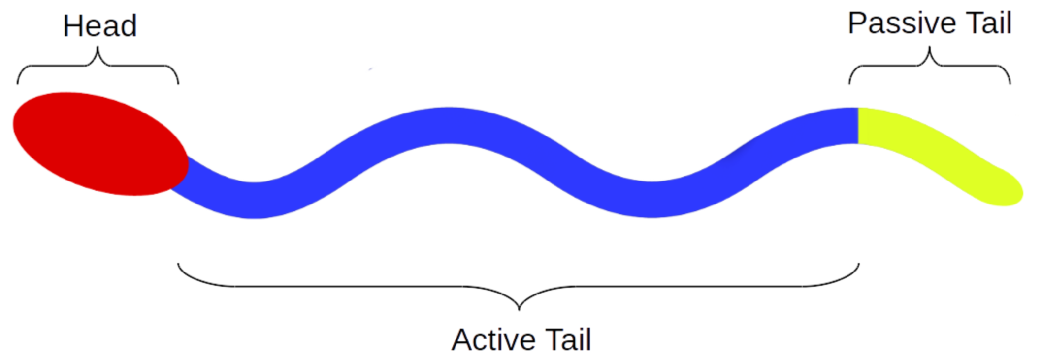
\includegraphics[scale=0.25]{images/swimmer-struc.png}
  \caption[Simbolic Swimmer Structure]{Simbolic Swimmer structure}
  \label{fig:Bild1}
  \end{footnotesize}
\end{figure} 


In this model, the swimmer consists on particles which are connected by bonds and are arranged in a filamentous structure. These particle-bonds connections have a bead-spring 
structure (Figure~\ref{fig:Bild2.4}). Initially, all particles in the tail ( active and passive fragments) has the same mass $m$. The bond length $l_{b}$ between neighboring
particles and the distance between the parallel filaments are identical. The filament length and the distance between filaments is described by harmonic bond potentials between
the two beads (spring constant K).\par

\begin{figure}[ht]
\centering
  \begin{footnotesize}
  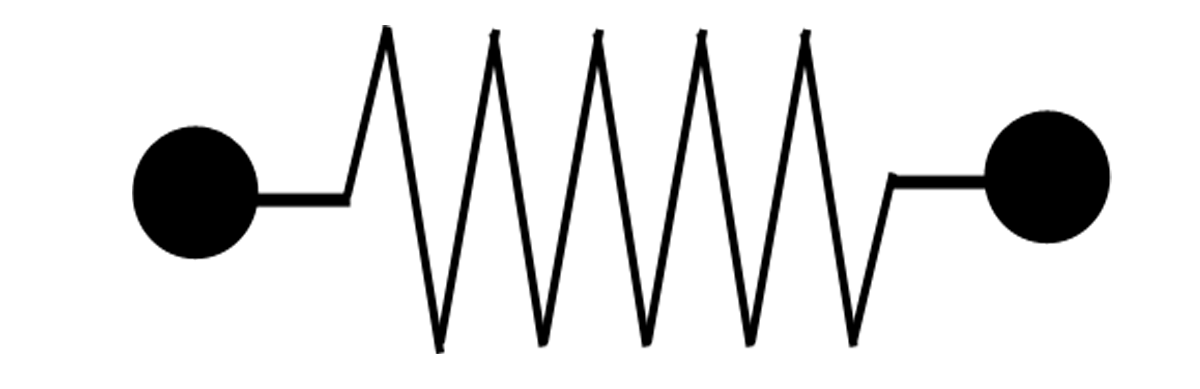
\includegraphics[scale=0.15]{images/bead-spring.png}
  \caption[Bead-Spring Structure]{Bead-Spring structure}
  \label{fig:Bild2.4}
  \end{footnotesize}
\end{figure} 

For the simulations, the swimmer has a total number of 100 particles, where three of those forms the swimmer head. Initially, it was used a square form for the head due to
simplifications, and after validating the method to create swimmers in LAMMPS, the swimmer was implemented with it final configuration which it is shown in Figure~\ref{fig:Bild2.5}.
In the final configuration the head has not a square format but an octagonal format which comes closer to the a circular/elliptical desired format.\par 
When the body starts to swim, the head takes a new format due to its mass properties. The fluid compress the head flesh turning it into a even more soft format getting closer to an 
ellipse and avoiding high corner angles(Figure~\ref{fig:Bild4}). It is also possible to observe in the sketch that the internal bonds get a new format when the swimmer starts to
deform into a wave format. This new format of the internal bonds gives a better mobility to the swimmer and avoid these bonds to break with deformation.  \par

\begin{figure}[ht]
\centering
  \begin{footnotesize}
  \includesvg{images/swimmer-compare-final}
  \caption[Initial swimmer structure configuration (upper) and modified final swimmer structure (lower)]{Initial swimmer structure configuration (upper) and modified final swimmer structure (lower)}
  \label{fig:Bild2.5}
  \end{footnotesize}
\end{figure} 

\begin{figure}[ht]
\centering
  \begin{footnotesize} 
  \includesvg{images/swimmer-moving}
  \caption[Swimmer deformed into a wave format with compressed head]{Swimmer deformed into a wave format with compressed head}
  \label{fig:Bild4}
  \end{footnotesize}
\end{figure} 

The harmonic bonds used to create the connections between the swimmer particles are applied in different ways thru the swimmer.Bonds are defined between specified pairs of 
atoms and remain in force for the duration of the simulation (unless the bond breaks which is possible in some bond potentials). The harmonic bond style uses the potential:


\begin{equation} 
  E = K ( r - r_{0})^2
\end{equation}

where $r_{0}$ is the equilibrium bond distance and $K$ is the bond stiffness constant. Note that the usual $1/2$ factor is included in $K$.

The internal bonds of the swimmer, that means the bonds which connects the upper and lower lines of the structure, have the aim to represent the swimmer backbones, so its 
physiological properties are different, and to represent it, the stiffness of those bonds are higher then the others in the swimmer borders. The passive bonds present in the 
rear of the tail are also harmonic and their lengths $l_{b}$ are constant. The active tail is formed by two lines of atoms connected by bonds, an upper and a lower line. Those
lines have a different bond type compared with the rest of the swimmer, as they are called active, the bond length is not constant in time. Changing the bond length it generates
a local spontaneous curvature. A sinusoidal variation of the bond length as a function of the contour length and time then generates the sinusoidal propagating wave of the active
lines. This approach is the most common in literature models, to prescribe the swimmer motion.\par

In Figure~\ref{fig:Bild2.7}, the red lines show the internal bonds with a higher stiffness relative with the rest of the swimmer, the blue points connected by the blue line show the 
head flesh which has an smaller mass and gets deformed as it swimms.\par
Many changes were applied in LAMMPS code as it was not ready to create specifically swimmers. Those changes are shown in the Chapter 3.


\begin{figure}[ht]
\centering
  \begin{footnotesize}
  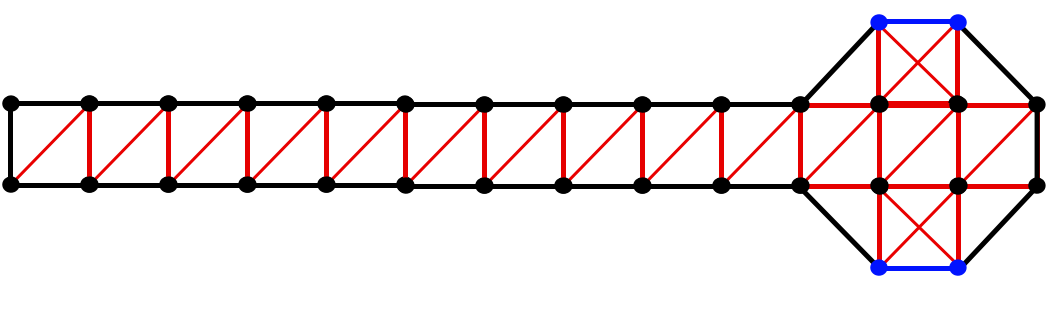
\includegraphics[scale=0.25]{images/swimmer-compare.png}
  \caption[Structure of the swimmer describing the internal bonds (red), the swimmer surface bonds (black) and the head flesh particles and bonds(blue)]{Structure of the swimmer describing the internal bonds (red), the swimmer surface bonds (black) and the head flesh particles and bonds (blue)}
  \label{fig:Bild2.7}
  \end{footnotesize}
\end{figure} 










\begin{figure}
\centering
  \begin{footnotesize}
  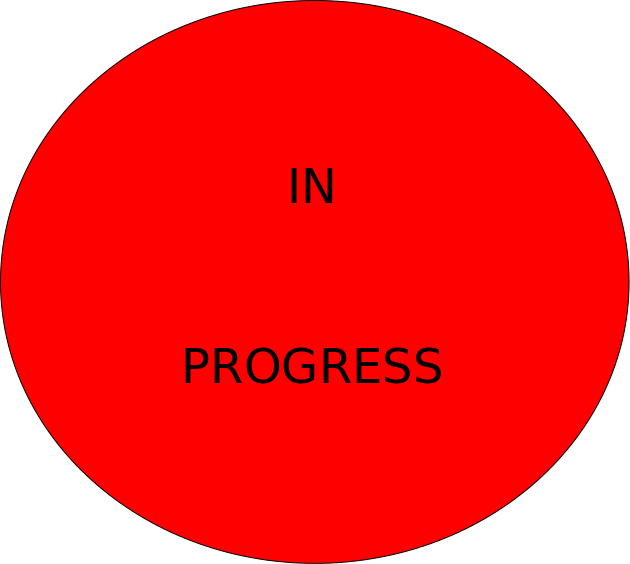
\includegraphics[scale=0.25]{images/in-progress.png}
  \caption[inprogress]{inprogress}
  \label{fig:Bild100}
  \end{footnotesize}
\end{figure} 

